Recently there has been a series of works related to assessing how synthetic data generators behave with data like the work of Emam et al. \cite{emamUtilityMetricsEvaluating2022} that especially focused on utility metrics for synthetic data generators. At the moment, comparing data is based on intra-columns and inter-columns relationship. The intracolumn relationship is assumed as something that compares equal columns between datasets, with highly known statistical methods like chi-squared or \ac{ks} like done in the works of \cite{combrinkComparingSyntheticTabular2022} among many others, acting more like sanity checks than anything else. 
Other known metrics are distance-based metrics like \ac{jsd}, Wasserstein Distance, Bhattacharyya Distance or Hellinger distance, which are based on the calculation of the distance between distributions like seen in the works of several teams \cite{ISI:000557358500024,choiGeneratingMultilabelDiscrete2017,Baowaly2019}.

However, regarding inter-column relationships, the metrics applied are often very different across papers. One example of trying to capture inter-column relationship is about the use of propensity score \cite{rosenbaumCentralRolePropensity1983,mullerEvaluationSyntheticElectronic2022} where a classifier is trained to the merged datasets, with the added variable of the original dataset (i.e., 1 for real and 0 for synthetic). The model is trained and the propensity Mean square error is the  mean squared difference of the estimated probability from the average prediction
Most recently, a unified metric appeared as the sum of other metrics known as described in the work of Chundawat et al., \cite{chundawatTabSynDexUniversalMetric2022}, known as TabSynDex. Other examples are likelihood of fitness like in the works of \cite{xuModelingTabularData2019b}, coverage support \cite{goncalvesGenerationEvaluationSynthetic2020a} or very specific metrics implemented for evaluating specific data generators.
However, the most used metric is cross-validation, which takes two datasets, one that is real and a second which is synthetic and we split both into train and test and train a machine learning model on the real data training set, then we test the model on both test sets. Then a ratio is created, rendering the actual value. This methodology, even if gold-standard at the moment for this type of study, has some liabilities since this value can be a bit erratic, and even above one since the evaluation metric could be better on the second dataset and we don't have a clear grasp of what that can represent in terms of dataset similarity. The image \ref{fig:1} represents this in detail. Several works used this metric as the comparing metric \cite{mullerEvaluationSyntheticElectronic2022}.

%TC:ignore
\begin{figure}[tbph]
\centering
\caption{Cross-Validation of datasets}\label{fig:1} 
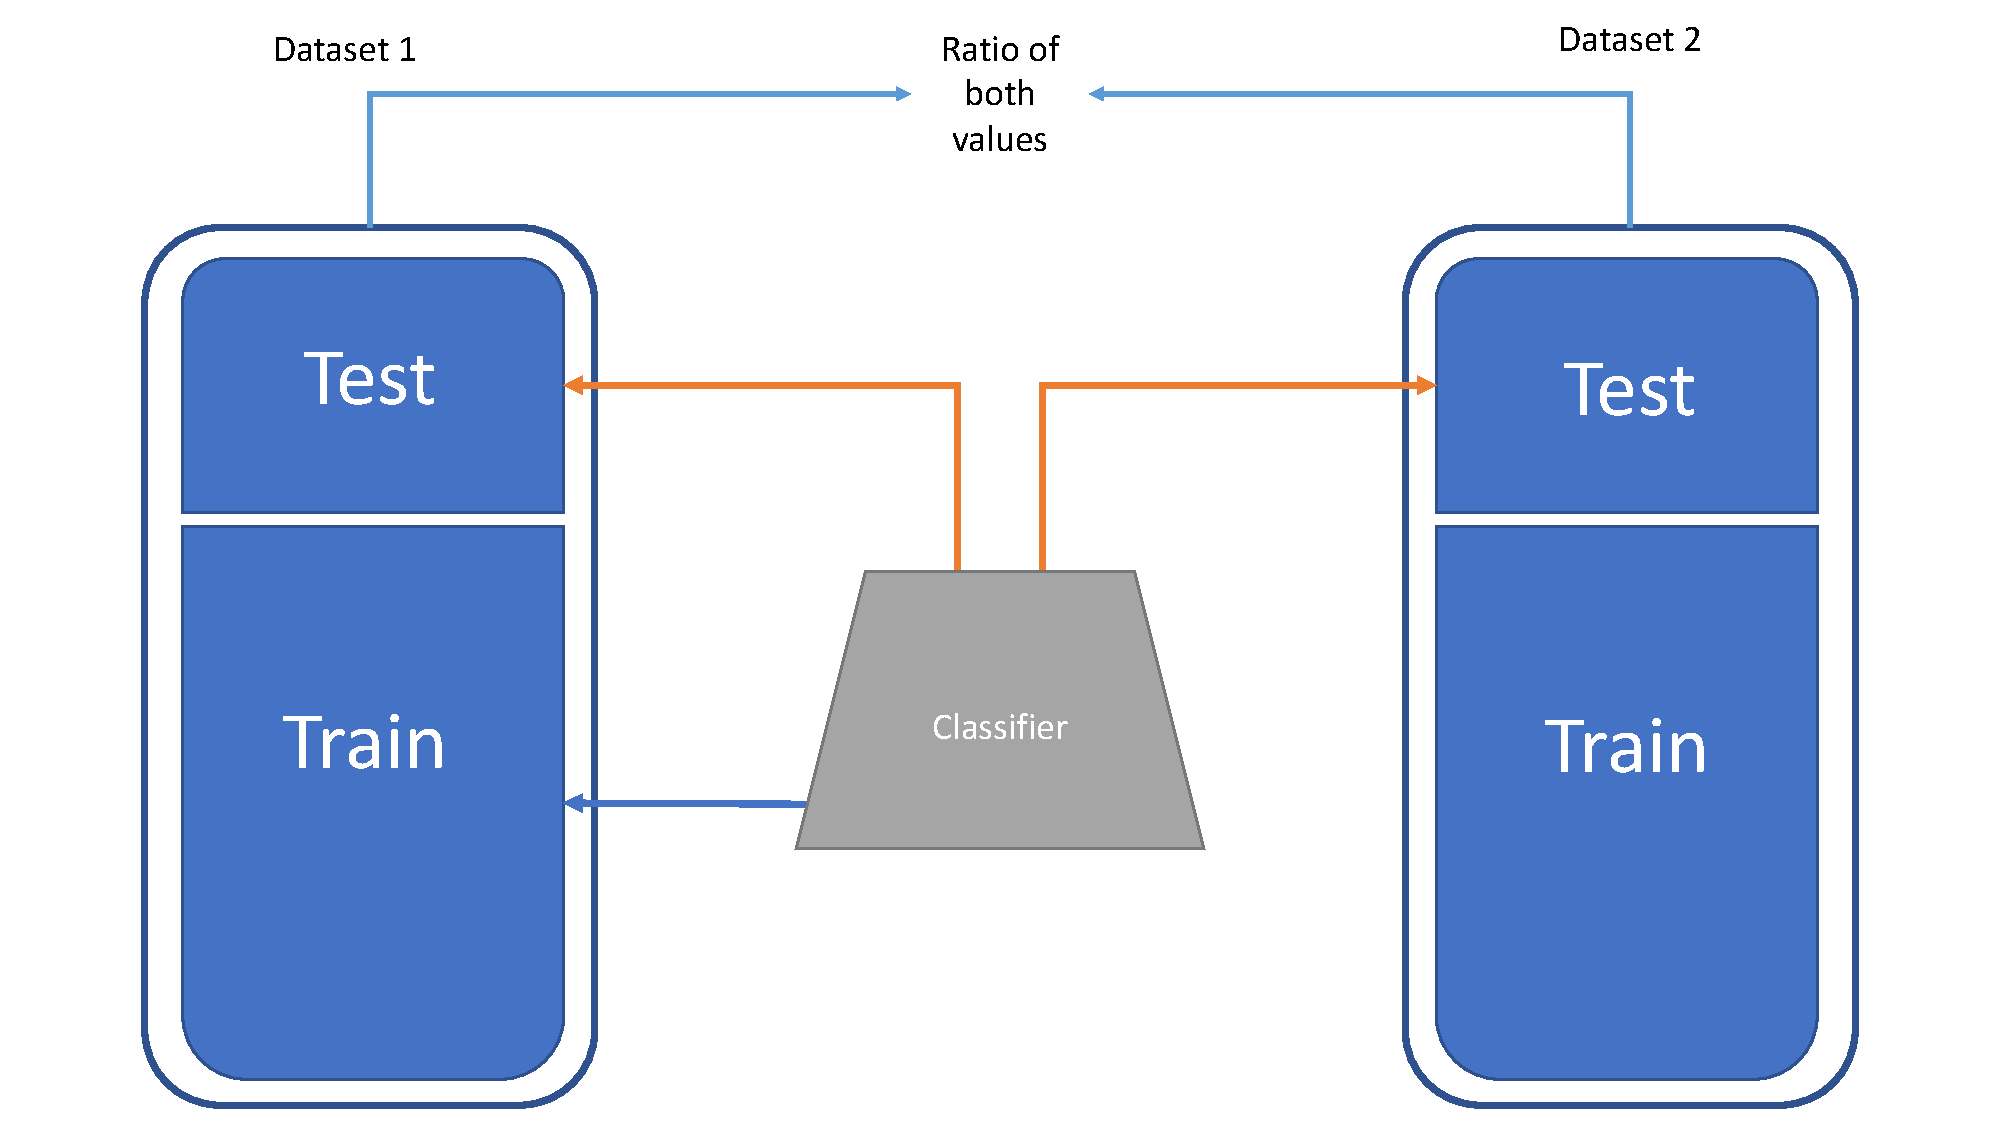
\includegraphics[scale=0.35]{figures/imagem1.pdf}
\end{figure}
%TC:endignore




%Utility Metrics for Evaluating Synthetic Health Data Generation Methods: Validation Study


